\resizebox{\textwidth}{!}{
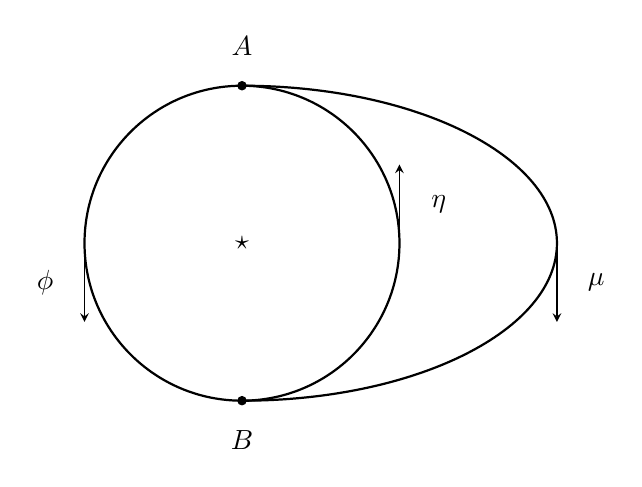
\begin{tikzpicture}
\draw[thick] (0,0) circle (2cm);
\draw (0,0) node {$\star$};

\draw[fill=black] (0,2) circle (1.5pt);
\draw (0,2.5) node {$A$};

\draw [-stealth] (2,0) -- (2,1);
\draw (2.5,0.5) node {$\eta$};

\draw[fill=black] (0,-2) circle (1.5pt);
\draw (0,-2.5) node {$B$};

\draw [-stealth] (-2,0) -- (-2,-1);
\draw (-2.5,-0.5) node {$\phi$};

%Primera distancia -> Eje horizontal
%Segunda distancia -> Eje vertical
\draw[thick] (0,2) arc (90:-90:4cm and 2cm);

\draw [-stealth] (4,0) -- (4,-1);
\draw (4.5,-0.5) node {$\mu$};
\end{tikzpicture}
}